\chapter{Interface 2 joueurs} \label{sec:chap1}
%Expliquer l'outil GUI
%Expliquer ce qui à été fait
%Expliquer organisation en classe et par bloc FMG
%Diagramme de classe ac E/S rôle
%Dans chaque bloc: explication détaillée
\section{Les règles du jeu}\label{sec:reglesDuJeu}
Commençons par définir les règles du jeu. Il y a deux objets (pions) dans le labyrinthe. L'un est représenté par pacman et l'autre par un fantôme. Le but de pacman est d'atteindre la sortie sans se faire attrapé plus de quatre fois par le fantôme. Le fantôme doit attraper pacman avant qu'il n'atteigne la sortie. Attention, si l'un des deux se retrouve bloqué entre quatre murs, il a perdu !\\
La partie se déroule comme suit : Les murs bougent (les murs verticaux vers le haut ou les murs horizontaux vers la droite), pacman bouge, le fantôme bouge. Il est interdit de rester sur place.\\
Nous avons dû définir ce que chacun connaît du système. Le labyrinthe est omniscient, il connaît les positions de chacun et l'ordonnancement. Pacman connait la position de la sortie et les murs autour de lui. Le fantôme ne connaît pas la sortie, connaît les murs autour de lui et peut voir pacman dans son couloir lorsqu'il n'est caché par aucun mur (oui il est très fort..).
\image{10cm}{1_Interface_2_joueurs/bloc_def.png}{Définition des ES connus pour chaque élément}




\section{L'interface}
\textit{Nous nous trouvons actuellement dans le dossier src/laby2players}\\
L'interface de base a été développée selon un modèle séquentiel et implémentée en langage objet avec Matlab. Voici son allure :
\image{15cm}{1_Interface_2_joueurs/explication_interface}{L'interface}
Sa création fût l'objet du premier bloc de projet.\\
L'interface a été réalisée grâce à la création de figure avec l'outil $GUI$ proposé par Matlab. Nous nous sommes beaucoup référé à l'aide Matlab pour comprendre et découvrir toutes les fonctionnalités offerte par la $GUI$


Le code est basé sur une implémentation par bloc FMG où chaque vecteurs d'entrées déterminera ce qui est connu par l'objet. Ces vecteurs d'entrées seront utilisés par le bloc F pour actualiser l'état du modèle, c'est à dire soit l'état des murs ou la position des objets dans le labyrinthe pour le \emph{Model Laby}, soit l'état de la commande pour les \emph{Model Walls}, \emph{Model Pacman} et \emph{Model Ghost}. 
%ca veut rien dire, à réecrire

Ensuite, chaque vecteur de sortie sera généré par le bloc G, en utilisant l'information sur l'état du système donnée par le bloc M. \\

\image{10cm}{1_Interface_2_joueurs/FMG.pdf}{Bloc FMG}
C'est $figure\_laby$ qui s'occupera de fera le lien entre l'utilisateur et les commandes automatiques. L'implémentation se déroule autour de plusieurs classes énumérée dans le diagramme de classe en figure \ref{fig:modelUML_GUI}
%insérer le diagramme de classe
\begin{figure}[!ht]
\centering
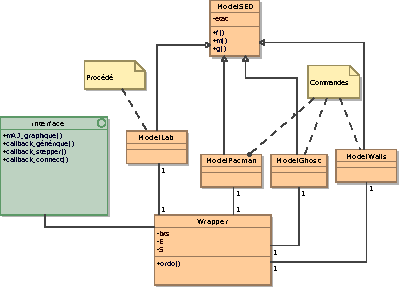
\includegraphics[width = \textwidth]{./1_Interface_2_joueurs/interactionModeles.pdf}
\caption{Modèle UML du GUI}\label{fig:modelUML_GUI}
\end{figure}
\section{Description des modèles} 
Vous trouverez dans cette section la description des modèles utilisés dans l'interface.
\subsection{ModelSED} 
Classe mère abstraite qui fait hérité les méthodes $f()$ $m()$ et $g()$ ainsi que les attributs $presentState$ et $initialState$ à toutes les classe filles qui sont : \begin{itemize}
\item [\textbullet] \emph{Model Ghost} qui permet de commander le fantôme. Vous trouverez la documentation des commandes implémenté dans \ref{sec:commandeGhost}
\item [\textbullet] \emph{Model Pacman} qui permet de commander le Pacman. Vous trouverez la documentation des commandes implémenté dans \ref{sec:commandePacman}
\item [\textbullet] \emph{Model Laby} décrit dans cette section.
\item [\textbullet] \emph{Model Walls} qui permet de commander le Walls. Vous trouverez la documentation des commandes implémenté dans \ref{sec:commandeMurs}
\item [\textbullet] \emph{Stop Condition} décrit aussi dans cette section.
\end{itemize}


\subsection{ModelLaby}\label{subsec:ModelLaby}
\begin{center}
Classe héritant de \emph{ModelSED} conntenue dans le fichier : /src/laby1player/ModelLaby.m et /src/laby2player/ModelLaby.m.
\end{center}
Classe héritant de ModelSED, on calcule les positions des murs et des objets entre chaque tour ici. Elle connaît également la sortie et le nombre de fois où pacman est attrapé. Elle est volontairement extrêmement condensée.
\paragraph*{Bloc F}
L'évolution de l'état du labyrinthe est effectué dans cette méthode : nous y calculons les matrices de murs et la position des objets en fonction des entrées du labyrinthe. Par exemple, si l'entrée \emph{Murs descendent} est activé, alors la fonction va renvoyer l'actualisation des matrices de murs.

Le format des entrées admises par cette fonction est dévellopé dans un vecteur de booléen. Il est défini en commentaire du code source de l'interface, dans le fichier \emph{figure\_laby.m}, dans le dossier \emph{laby1player} ou \emph{laby2player}, dans la fonction \textit{function ui\_Callback(hObject, eventdata, handles)}. 
%bloc F je ne comprends pas
\paragraph*{Bloc M}
Nous actualisons l'état présent du modèle en fonction de celui calculé dans la fonction $f$. Pour cela, vous devez le mettre dans les inputs de la fonction. La méthode attend aussi un booléen pour lui indiquer si le modèle doit être remis à l'état initial.\\
%Quoi ????

Il est à noter que le calcul du compteur $caught$, c'est à dire le compteur du nombre de fois qu'a été attrapé le Pacman \ref{sec:reglesDuJeu}, est aussi effectué dans cette méthode (dans la version 2 joueurs). Pour cela, nous faisons appel aux positions des deux objets et à la connaissance des murs, pour inspecter qu'il n'y a pas de murs entre les deux objets.


\paragraph*{Bloc G} La fonction de génération des sorties est implémentée dans la méthode portant ce nom. Nous allons dans la liste ci dessous vous détailler l'ensemble des sorties de ce modèle et expliquer la méthode de calcul utilisée.  \begin{itemize}
\item [\textbullet] \underline{Murs autour d'un objet :} Permet d'identifier quel(s) mur(s) (Haut, Bas, Gauche et/ou Droite) sont autour d'un objet. Ces sorties sont représentées sur un vecteur identique pour tous les objets, décrit dans le constructeur de la classe "Wrapper", qui est mis à VRAI si un mur se trouve dans la direction et 0 sinon.
\item [\textbullet] \underline{Pacman est sur la sortie :} En fonction de la position de l'objet PACMAN et de la position de la sortie ESCAPE, détermine si l'objet est sorti ou non du labyrinthe.
\item [\textbullet] \underline{Le ghost voit le Pacman:} (Uniquement dans la version 2 joueurs) Si les positions des objets Pacman et Ghost ont le même $x$ ou le même $y$, et qu'aucun mur ne se trouve entre les deux, alors le ghost peut voir le pacman. Comme pour le vecteur "Murs autour d'un objet", cette sortie est représentée sur un vecteur où chaque élément indique une direction et est mis à 1 quand la vue du pacman par le ghost est VRAI, 0 sinon.
\end{itemize}

\subsection{StopCondition}\label{subsec:StopCondition}
\begin{center}
Classe héritant de \emph{ModelSED} conntenue dans le fichier : /src/laby1player/StopCondition.m et /src/laby2player/StopCondition.m.
\end{center}
Cette classe permet d'établir l'arrêt du labyrinthe. Pour cela, elle admet en entrée les 2 (ou 4 pour labyrinthe à 2 joueurs) paramètres qui permettent d'arrêter le modèle du labyrinthe : \begin{itemize}
\item [\textbullet] \emph{noEscape} variable booléenne qui indique si le Pacman se trouve sur la sortie.
\item [\textbullet] \emph{pacmanWallsBreak} vecteur contenant les murs autour du Pacman.
\item [\textbullet] \emph{ghostWallsBreak} (pour labyrinthe à 2 joueurs) vecteur contenant les murs autour du Ghost.
\item [\textbullet] \emph{caught} (pour labyrinthe à 2 joueurs) entier représentatn le nombre de fois que le Pacman a été capturé par le Ghost.
\end{itemize}
Elle contient aussi une évolution sous forme de bloc "FMG" décrite précédemment. 

\section{Description du "Wrapper"}\label{sec:Wrapper}
\begin{center}
Nous allons dans cette partie détaillé les fichiers \emph{wrapper.m}. Vous les trouverez les sources dans : \textit{src/laby1player} et \textit{src/laby2player}.
\end{center}
Cette section est entièrement dédié aux explications sur la classe \emph{Wrapper}. Vous y trouverez dans un premier temps une description des attributs contenu dans la classe puis nous détaillerons dans 3 sous-sections les méthodes importantes.
\subsection{Attributs du Wrapper}
La description des attributs de cette classe se situe en début du code source de la classe. Nous avons placé dans cette liste d'attributs l'ensemble des états des modèles connectés par le "Wrapper" : \emph{ModelLaby}, \emph{commandWalls}, \emph{commandPacman}, \emph{stopCondition} et \emph{commandGhost} (pour le labyrinthe 2 joueurs). Nous y avons aussi placé une variable servant de compteur : \emph{whoPlay}. Elle permettra de connaître, selon l'ordonnancement, quel modèle doit être appelé. 


Cette classe contient également 2 (ou 3 pour 2 joueurs) attributs booléen pour la connection des commandes automatique. Ces variables ont pour fonctions d'activer le mode de fonctionnement automatique du labyrinthe. Elles sont mise à jour dans la fonction \emph{updateConnexion} que nous décrivons en détail dans \ref{subsec:majConnexion} et sont utilisées dans la fonction \emph{orderer} décrite en \ref{subsec:orderer}. 


Enfin, la classe possède deux attributs permettant le bon fonctionnement des connexions : il s'agit de \emph{in} et \emph{out}. Ce vecteur et cette cellule (respectivement) ont le rôle de médium entre les modèles : la cellule \emph{out} va contenir les sorties du labyrinthe (i.e les sorties de la classe \emph{ModelLaby}) pour les envoyer en entrées aux modèles de commandes. Le vecteur \emph{in} va quand à lui contenir les sorties des commandes pour qu'elles puissent être envoyé au labyrinthe. Ces 2 derniers attributs sont sous utilisé dans la méthode décrite en \ref{subsec:orderer}. 


Les initialisations de ces attributs sont effectuées dans le constructeur de la classe. Nous attirons votre attention sur l'instanciation des attribuits contenant les instances des modèles : ceux-ci ont besoin de recevoir leur état initial. Celui ci sera stocké dans chaque modèle et ne pourra être changer au cours de l'éxécution du programme.  

\paragraph*{Remarque} Les initialisations des paramètres du labyrinthe peuvent être modifiés lors de la construction de l'objet \emph{wrapper}, dans la fonction \emph{figure\_Laby\_OpeningFcn} appartenant à l'interface Graphique. Elle est donc contenu dans le fichier \emph{figure\_laby.m}, situé dans le même dossier que le fichier qui vous présenté en ce moment.
\subsection{Mise à jour des connexions}\label{subsec:majConnexion}
Cette méthode s'appelle \emph{updateConnexion} et a pour fonction d'actualiser les 2 (ou 3) booléens de connexion. Pour donner un exemple de son fonctionnement, quand un utilisateur clique sur le bouton connexion depuis l'interface présenté en \ref{L'interface}, l'interface appelle cette fonction pour mettre à jour le bit de connexion. 

\subsection{Initialisation du labyrinthe}\label{subsec:initLab}
Nous avons rapidement été confronté au problèmes de ré-initialisation de notre labyrinthe : chaque modèle devait rappeler son état initial en même temps. Nous avons donc choisi de créer cette méthode qui permet d'appeler tout les méthodes \emph{m} des modèles SED et de lancer l'initialisation de chaque modèle. Pour rappel, les méthodes \emph{m} permettent de mémoriser l'état du labyrinthe comme le montre le schéma en \ref{Bloc FMG}.

\subsection{Ordonnancement des modèles}\label{subsec:orderer}
%Comme son nom l'indique c'est lui qui gère l'ordonnancement des actions. C'est ici qu'on implémente les tours de jeux (d'abord les murs puis le Pacman puis le fantôme). Il gère également le mode manuel/automatique/semi-manuel/ à l'aide de ces attributs. 
Pour permettre le bon ordonnancement d'appel des modèles, nous avons développé une méthode nommé \emph{orderer}. C'est dans cette fonction que nous avons implémenté les tours de jeux : d'abord les murs puis le Pacman (et le Ghost pour le labyrinthe à 2 joueurs) avec entre chaque une mise a jour du labyrinthe. Cet ordonnancement est géré grâce à l'attribut \emph{whoPlay} que nous vous présentions en début de section : il prend la valeur 0 ou 1 (ou 2 dans le cas 2 joueurs) pour connaître quel modèle doit être appelé : murs ou Pacman (ou Ghost) respectivement.
 

La méthode gère également le mode manuel/automatique/semi-manuel/ à l'aide de ces attributs \emph{\underline{objet}bit} : si ce bit de connexion n'est pas à 1, alors la méthode ne fait pas appel au modèle correspondant. Dans ce cas, le vecteur \emph{in} qui est envoyé au labyrinthe est celui construit par l'interface. Sinon, le modèle de l'objet connecté est instancié : appel des méthodes \emph{f}, \emph{m} puis \emph{g} de celui-ci.

\paragraph*{Remarque} Les entrées des modèles des murs et des objets est contenu dans la cellule \emph{out}. il est donc possible de modifier les entrées possibles de chaque modèle au niveau des appels des méthodes \emph{f} de chaque modèle. 



 

